\section{Gruppen}
\begin{definition}
	Eine \textbf{Gruppe} $(G, *)$ ist eine Menge $G$ mit einer binären Verknüpfung 
	\[* \colon G \times G \to G, (g,h) \mapsto g*h,\]
	so dass gilt:
	\begin{enumerate}[label={\bfseries(G\arabic*)}]
		\item $(a * b) * c  = a * (b * c)$ für alle $a,b,c \in G$ ($*$ assoziativ),
		\item Es existiert ein $e \in G$, sodass für alle $a \in G$ gilt $a * e = a = e * a$ ($e$ neutrales Element),
		\item Für alle $a \in G$ existiert ein $a' \in G$, sodass $a * a' = e = a' * a$ ($a'$ inverses Element zu $a$).
	\end{enumerate}
	Gilt zusätzlich
	\begin{enumerate}[start=4, label={\bfseries(G\arabic*)}]
		\item $a * b = b * a$ für alle $a,b \in G$, so heißt $(G, *)$ \textbf{kommutativ} oder \textbf{abelsch}.
	\end{enumerate}
	Die \textbf{Ordnung} von $(G, *)$ ist $|G|$.
\end{definition}
\underline{Notation: } Wir schreiben meist $G$ statt $(G, *)$. Dabei ist $*$ oft entweder $+$ (\textbf{additive Gruppe}) oder $\cdot$ (\textbf{multiplikative Gruppe}). Dann schreibe 0 statt $e$ bzw. $-a$ statt $a'$ sowie $a-b := a + (-b)$, schreibe 1 statt $e$ bzw. $a^{-1}$ statt $a'$ sowie $ab := a \cdot b$.
\begin{rem}\label{rem1_2}
	\begin{enumerate}[label=(\roman*)]
		\item Das neutrale Element einer Gruppe $G$ ist eindeutig:
		
		Sind $e, f$ neutrale Element in $G$, so gilt $e = e * f = f$ nach (G2).
		
		\item Inverse Elemente in $G$ sind eindeutig:
		
		Seien $a'$ und $a''$ Inverse zu $a \in G$. Dann gilt
		\[a' \overset{(G2)}{=}  a' * e \overset{(G3)}{=} a' * (a * a'') \overset{(G1)}{=}  ( a' * a) * a'' \overset{(G3)}{=} = e * a'' \overset{(G2)}{=} a''\]
		
		\item Für inverse Elemente in $G$ gilt $(a')' = a$ und $(a * b)' = b' * a'$.
	\end{enumerate}
	\begin{beispiel}\label{beispiel1_3}
		\begin{enumerate}
			\item $(R, +, \cdot)$ ein Ring $\implies$ $(R, +)$ abelsche Gruppe.
			
			 $(K, +, \cdot)$ ein Körper $\implies$ $(K, +)$ und $(K\setminus \{0\}, \cdot)$ abelsche Gruppe
			 
			$(V, +, \cdot)$ ein Vektorraum $\implies$ $(V, +)$ abelsche Gruppe.
			
			Zum Beispiel $V = M_n (K) := \{ n\times n\text{-Matrizen über einem Körper } K\}$.
			
			\item $\mathrm{GL}_n(K) := \{\text{invertierbare } n\times n\text{-Matrizen über einem Körper } K\}$ bildet eine Gruppe bzgl. Matrizenmultiplikation - die \textbf{allgemeine lineare Gruppe}. Diese ist für $n \geq 2$ nicht abelsch. 
			
			Weitere Beispiele: 
			\begin{itemize}
				\item $\mathrm{SL}_n(K) := \{A \in \mathrm{GL}_n(K) \mid \det A = 1\}$ - die \textbf{spezielle lineare Gruppe}.
				\item $\mathrm{O}_n(K) := \{A \in \mathrm{GL}_n(K) \mid AA^\top = E_n\}$ - die \textbf{orthogonale Gruppe}.
			\end{itemize}
			
			\item $G = \{e\}$ ist die \textbf{triviale Gruppe}.
			
			Für $|G| = 2$ mit $G = \{1, g\}$, dann erhalten wir die eindeutige \textbf{Multiplikationstafel}:
			
			\begin{center}
				\begin{tabular}{c|cc}
					$\cdot$ & 1 & $g$ \\
					\hline
					1 & 1 & $g$ \\
					$g$ & $g$ & 1
				\end{tabular}
			\end{center}
				Für $|G| = 3$ mit $G = \{1, g, h\}$, dann erhalten wir die eindeutige Multiplikationstafel:
				\begin{center}
					\begin{tabular}{c|ccc}
						$\cdot$ & 1 & $g$ & $h$\\
						\hline
						1 & 1 & $g$ & $h$\\
						$g$ & $g$ & $h$ &  1\\
						$h$ & $h$ & 1 & $g$
					\end{tabular}
				\end{center}
				Für $|G| = 4$ wird es schwieriger.
			
			\item \textbf{Symmetriegruppen: } Sei $G$ die Menge der \textbf{Kongruenzabbildungen} (längenerhaltend, flächenerhaltend, winkelerhaltend) eines geometrischen Objektes auf sich selbst.
			%Bild			
			\item Sei $X \neq \emptyset$ eine Menge. Die \textbf{symmetrische Gruppe} auf $X$ ist gegeben durch $S_X = \{f\colon X \to X \mid f \text{ bijektiv}\}$ mit der gewöhnlichen Komposition von Abbildungen. 
			
			Für $X = \{1, \dots, n\}$ mit $n \in \N$ erhalten wir die \textbf{symmetrische Gruppe vom Grad $n$} und schreiben $S_X = S_n$. 
			
			Die Elemente in $S_n$ heißen \textbf{Permutationen} und es gilt 
			\[|S_n| = n!.\]
			
			\textbf{Matrixnotation: } Die Permutation $\sigma \colon \{1, \dots, n\} \to \{1, \dots, n\}$ mit $\sigma(i) = a_i$ für $1 \leq i \leq n$ schreiben wir auch als
			\[\sigma = \begin{pmatrix}
				1 & 2 & 3 & \dots & n\\
				a_1 & a_2 & a_3 & \dots & a_n
			\end{pmatrix}.\]
			
			\textbf{Zykelnotation: } Sei $\{a_1, \dots, a_r\} \subseteq \{1, \dots, n\}$ mit $a_i$ paarweise verschieden. Dann ist der \textbf{Zykel} $\sigma = (a_1, \dots, a_r)$ \textbf{der Länge $r$} definiert als die Permutation $\sigma \in S$ mit 
			\begin{align*}
				\sigma(a_1) &= a_2\\
				\sigma(a_2) &= a_3\\
				&\vdots\\
				\sigma(a_r) &= a_1\\
			\end{align*}
			und $\sigma(a) = a$ für alle $a \in \{1, \dots, n\} \setminus \{a_1, \dots, a_r\}$. Zykel der Länge 2 heißen \textbf{Transpositionen}. Zwei Zykel $(a_1 \dots a_r)$ und $(b_1 \dots b_s)$ heißen \textbf{disjunkt}, falls 
			\[\{a_1, \dots, a_r\} \cap \{b_1, \dots, b_r\} = \emptyset.\]
			Disjunkte Zykel kommutieren und jede Permutation lässt sich eindeutig als Komposition disjunkter Zykel schreiben.
			
			Zum Beispiel 
			\[\sigma = \begin{pmatrix}
				1 & 2 & 3 & 4 & 5\\
				3 & 4 & 1 & 5 & 2
			\end{pmatrix}\]
			entspricht der Permutation $(13)(245)$ in Zykelschreibweise.
			
			\item Seien $G$ und $H$ Gruppen. Dann wird auch $G \times H$ zu einer Gruppe durch
			\[(g_1, h_1) * (g_2, h_2) := (g_1 *_G g_2, h_1 *_H h_2).\]
			$G \times H$ heißt das \textbf{direkte Produkt} von $G$ und $H$.
		\end{enumerate}
	\end{beispiel}
\end{rem}
\begin{definition}
	Seien $G$ und $H$ Gruppen
	\begin{enumerate}[label=(\alph*)]
		\item Eine Abbildung $\varphi \colon G \to H$ heißt \textbf{Gruppenhomomorphismus}, falls 
		\[\varphi(g_1 *_G g_2) = \varphi(g_1) *_H \varphi(g_2)\]
		für alle $g_1, g_2 \in G$. Ist $\varphi$ auch bijektiv, sprechen wir von einem \textbf{Isomorphismus}. Die Gruppen $G$ und $H$ heißen dann \textbf{isomorph} und wir schreiben $G \cong H$.
		\item $H$ heißt \textbf{Untergruppe} von $G$, falls $H \subseteq G$ und die Inklusionsabbildung $H \to G$ ein Gruppenhomomorphismus ist. Wir schreiben $H \leq G$.
	\end{enumerate}
\end{definition}

\begin{rem}
	\begin{enumerate}[label=(\roman*)]
		\item Sei $\varphi \colon G \to H$ ein Gruppenhomomorphismus. Dann gilt
		\[\varphi(1_G) = 1_H,\]
		denn es gilt
		\[\varphi(1_G) = \varphi(1_G 1_G) = \varphi(1_G) \varphi(1_G)\]
		und Multiplikation mit $\varphi(1_G)^{-1}$ liefert 
		\[1_H = \varphi(1_G).\]
		
		Zudem gilt
		\[\varphi(g^{-1}) = \varphi(g)^{-1},\]
		denn
		\[\varphi(g) \varphi(g^{-1}) = \varphi(gg^{-1}) = \varphi(1_G) = 1_H = \dots = \varphi(g^{-1}) \varphi(g).\]
		Nutze Bemerkung \ref{rem1_2} (ii) zum Beweis der Eindeutigkeit.
		
		\item Isomorphie ist eine Äquivalenzrelation. Isomorphe Gruppen betrachten wir als wesensgleich, in Hinblick auf Eigenschaften, Multiplikationstafeln, Eindeutigkeitsaussagen etc.
		
		\item Sei $G$ eine Gruppe und $H \subseteq G$. Dann ist $H \leq G$ Untergruppe genau dann, wenn 
		\begin{itemize}
			\item $1_G \in H$,
			\item $h_1, h_2 \in H \;\Rightarrow\; h_1h_2 \in H$,
			\item $h \in H \;\Rightarrow\; h^{-1} \in H$.
		\end{itemize}
	\end{enumerate}
\end{rem}

\begin{beispiel}\label{beispiel1_6}
	\begin{enumerate}
		\item $\det \colon \GL_n(K) \to K \setminus \{0\}$ ist ein Gruppenhomomorphismus, da $\det(AB) = \det(A)\det(B)$ für alle $A,B \in \GL_n(K)$. $\SL_n(K) \leq \GL_n(K)$ und $\mathrm{O} \leq \GL_n(K)$ sind Untergruppen.
		
		\item $\exp \colon \R \to \R_{>0}$ ist ein Gruppenisomorphismus, da $\exp(x+y) = \exp(x)\exp(y)$ für alle $x,y \in \R$.
		
		\item Sei $G = \{\id, \gamma_A, \gamma_B\}$ die Symmetriegruppe eines Rechtecks wie in Beispiel \ref{beispiel1_3} (4). Dann ist $G$ isomorph zum direkten Produkt $S_1 \times S_2$. Ein Isomorphismus ist gegeben durch $G \to S_1 \times S_2$ mit
		\begin{align*}
			\id &\mapsto (\id, \id)\\
			\gamma_A &\mapsto (\id, (12))\\
			\gamma_B &\mapsto ((12), \id)\\
			\gamma_{180^\circ} &\mapsto ((12), (12))
		\end{align*}
		\textbf{vergleiche Multiplikationstafeln}.
		
		\item Für $n \in \N$ ist $\varphi \colon S_n \to S_{n+1}$ mit 
		\[\varphi(\sigma) = \begin{pmatrix}
			1 & \dots & n & n+1\\
			\sigma(1) & \dots & \sigma(n) & n+1
		\end{pmatrix}\]
		ein injektiver Gruppenhomomorphismus, d.h. $S_n$ ist isomorph zu einer Untergruppe von $S_{n+1}$.
		
		\item Sei $G$ eine Gruppe und $g \in G$. Dann ist die Abbildung 
		\[C_g \colon G \to G, \quad h \mapsto ghg^{-1},\]
		genannt \textbf{Konjugation mit $g$}, ein Gruppenisomorphismus mit
		\[(C_g)^{-1} = C_{g^{-1}}.\]
		Die Abbildungen
		\begin{align*}
			L_g &\colon G \to G, \quad h \mapsto gh\\
			R_g &\colon G \to G, \quad h \mapsto hg,
		\end{align*}
		genannt \textbf{Links-} und \textbf{Rechtsmultiplikation mit $g$}, sind im Allgemeinen keine Gruppenhomomorphismus, aber bijektiv!
		
		\item Sei $\varphi \colon G \to H$ ein Gruppenhomomorphismus. Dann sind $Ker(\varphi) := \{g \in G \mid \varphi(g) = 1_H\}$ (\textbf{Kern von $\varphi$}) und $\im(\varphi) = \{\varphi(g) \mid g \in G\}$ (\textbf{Bild von $\varphi$}) Untergruppen von $G$ bzw. $H$. Zudem ist $\varphi$ injektiv genau dann, wenn $Ker(\varphi) = \{1_G\}$.
		
		\begin{proof}
			\glqq{}Nur dann\grqq: Sei $g \in G$ mit $\varphi(g) = 1_H$. Da $\varphi(1_G) = 1_H$, folgt $g = 1_G$.
			
			\glqq{}Dann\grqq: Seien $a,b \in G$ mit $\varphi(a) = \varphi(b)$. Da $1_H = \varphi(a) \varphi(b)^{-1} = \varphi(ab^{-1})$, folgt $ab^{-1} = 1_G$ und somit $a = b$.
		\end{proof}
	\end{enumerate}
\end{beispiel}

\begin{satz}[Satz von Cayley]\label{satz1_7}
	Jede Gruppe ist isomorph zu einer Untergruppe einer symmetrischen Gruppe, d.h. einer Gruppe von Bijektionen.
\end{satz}
\begin{proof}
	Sei $G$ eine Gruppe. Wir konstruieren einen injektiven Gruppenhomomorphismus $\varphi \colon G \to S_G = \{f \colon G \to G \mid f \text{ bijektiv}\}$ durch $g \mapsto L_g$ (siehe Beispiele \ref{beispiel1_3} (5) und \ref{beispiel1_6} (5)). 
	
	\underline{Z.z.: $\varphi$ ist Gruppenhomomorphismus.} Seien $g, h \in G$. Dann gilt für alle $a \in G$
	\begin{align*}
		\varphi(gh)(a) = L_{gh}(a) = (gh)(a) = g(ha) = L_g(ha) = (L_g \circ L_h)(a) = (\varphi(g) \circ \varphi(h))(a)
	\end{align*} 
	und somit $\varphi(gh) = \varphi(g) \circ \varphi(h)$. 
	
	\underline{Z.z.: $\varphi$ ist injektiv:} Seien $g,h \in G$ mit
	\[L_g = \varphi(g) = \varphi(h) = L_h.\]
	Dann gilt 
	\[g = L_g(1_G) = L_h(1_G) = h.\]
	Ist $G$ endlich mit $|G| = n$, so ist $G$ isomorph zu einer Untergruppe von $S_n$, der symmetrischen Gruppe vom Grad $n$.
\end{proof}
% Vorlesung 21.10.2024:
\begin{beispiel}\label{beispiel1_8}
	Für $\sigma \in S_n$ definiere $\sgn(\sigma) = (-1)^{\omega(\sigma)}$, wobei 
	\[\omega(\sigma) = \left|\{(i,j) \mid 1 \leq i < j \leq n, \sigma(j) < \sigma(i)\}\right|,\]
	genannt die \textbf{Anzahl der Fehlstände von $\sigma$}. Dann ist
	\[\sgn(\sigma) = \prod_{i < j} \frac{\sigma(i) - \sigma(j)}{i - j}.\]
	Zum Beispiel ist für 
	\[\sigma = \begin{pmatrix}
		1 & 2 & 3 \\
		3 & 2 & 1
	\end{pmatrix}\]
	das Signum
	\[\sgn(\sigma) = \frac{3-2}{1-2} \cdot \frac{3-1}{1-3} \cdot \frac{2-1}{2-3} = (-1)^3 = -1.\]
	$\sigma$ hat 3 Fehlstände. Die Abbildung $\sgn \colon S_n \to (\{-1, 1\}, \cdot)$ ist ein Gruppenhomomorphismus, da für $\sigma, \pi \in S_n$ gilt
	\[\sgn(\sigma \pi) = \prod_{i < j} \frac{\sigma(\pi(i)) - \sigma(\pi(j))}{i - j} = \prod_{i < j} \frac{\sigma(\pi(i)) - \sigma(\pi(j))}{\pi(i) - \pi(j)} \cdot \prod_{i < j} \frac{\pi(i) - \pi(j)}{i - j} = \sgn(\sigma) \cdot \sgn(\pi)\]
	Nach Beispiel \ref{beispiel1_6} (6) ist $A_n := \ker(\sgn)$ Untergruppe von $S_n$. $A_n$ heißt die \textbf{alternierende Gruppe vom Grad $n$}.
	
	Zum Beispiel ist für $S_3 = \{\id, (12), (13), (23), (123), (132)\}$: 
	\[A_3 = \{\id, (123), (132)\}.\]
\end{beispiel}
\begin{definition}
	Sei $G$ eine Gruppe und $H \leq G$. Für $g \in G$ heißt
	\begin{align*}
		gH &:= \{gh \mid h \in H\} &&\textbf{(Linksnebenklasse von $H$ in $G$)}\\
		Hg &:= \{hg \mid h \in H\} &&\textbf{(Rechtsnebenklasse von $H$ in $G$)}
	\end{align*}
	Schreibe $G / H = \{gH \mid g \in G\}$ und $H \backslash G = \{Hg \mid g \in G\}$. Definiere $[G : H] := \left|\sfrac{G}{H}\right|$.
\end{definition}
\begin{rem}
	\begin{enumerate}[label=(\roman*)]
		\item Nach Beispiel \ref{beispiel1_6} (5) gilt
		\[|gH| = |H| = |Hg|\]
		für alle $g \in G$.
		\item Nach Aufgabe M.1.3 definieren die Relationen $a \sim_1 b \Leftrightarrow a^{-1}b \in H$ bzw. $a \sim_2 b \Leftrightarrow ab^{-1} \in H$ Äquivalenzrelationen auf $G$. Die Äquivalenzklassen sind genau die Links- bzw. Rechtsnebenklassen von $H$ in $G$.
		
		Insbesondere gilt 
		\begin{align*}
			G &= \bigcup_{g \in G} gH = \bigsqcup_{N \in G/H} N,\\
			G &= \bigcup_{g \in G} Hg = \bigsqcup_{N \in H \backslash G} N
		\end{align*}
		\begin{proof}
			Für $[a] = \{b \mid a_1 \sim_1 b\}$ gilt: $b \in [a] \Leftrightarrow a^{-1}b \in H \;\Leftrightarrow\; \exists h \in H : a^{-1}b = h \;\Leftrightarrow\; \exists h \in H : b = ah \;\Leftrightarrow\; b \in aH$.
		\end{proof}
	\end{enumerate}
\end{rem}
\begin{satz}[Satz von Lagrange]\label{satz1_11}
	Sei $G$ eine endliche Gruppe und $H \leq G$. Dann gilt
	\[|G| = [G : H] \cdot |H|.\]
	Insbesondere also $|H| \big| |G|$ ($|H|$ teilt $|G|$).
\end{satz}
\begin{proof}
	Wähle $\{g_1, \dots, g_r\} \subseteq G$, so dass
	\[G = \bigsqcup_{j=1}^r g_i H\]
	gilt, d.h. $[G:H] = r$. Dann gilt
	\[|G| = \sum_{j=1}^{r} |g_jH| = \sum_{j=1}^r |H| = r|H| = [G:H] \cdot |H|.\]
\end{proof}
\begin{center}
	Definiert $g_1H * g_2H := g_1g_2H$ eine Gruppenstruktur auf der $G/H$?
\end{center}
\underline{Problem:} Wohldefiniertheit.
\begin{beispiel}
	Sei $G = S_3$ und $H = \{\id, (12)\}$. Da $|G|= 6$ und $|H| = 2$, folgt mit Satz \ref{satz1_11}, dass $[G:H] = 3$. Es gibt also 3 Linksnebenklassen:
	\[\id H = H, \quad (23)H = \{(23), (132)\} \quad\text{und}\quad (13)H = \{(13), (123)\}\]
	Wir erhalten
	\[(23)H * (13)H = (123)H\]
	und
	\[(23)H = (132)H * (13)H = (12)H.\]
	$(123)H \neq (12)H$ und wir folgern:
	
	Wir brauchen eine stärkere Bedingung als $H \leq G$ Untergruppe.
\end{beispiel}
\begin{definition}
	Sei $G$ eine Gruppe und $H \leq G$. 
	\begin{enumerate}[label=(\alph*)]
		\item Für $g \in G$ heißt $gHg^{-1} = \{ghg^{-1} \mid h \in H\}$ die \textbf{zu $H$ konjugierte Untergruppe}. Nach Beispiel \ref{beispiel1_6} (5), (6) gilt $gHg^{-1} \leq G$ mit $|gHg^{-1}| = |H|$ für alle $g \in G$.
		\item $H \leq G$ heißt \textbf{normale Untergruppe} oder auch \textbf{Normalteiler}, falls 
		\[gHg^{-1} = H \quad\text{für alle } g \in G.\]
		Wir schreiben $H \unlhd G$.
	\end{enumerate}
\end{definition}
\begin{rem}\label{rem1_14}
	Die folgenden Aussagen sind äquivalent
	\begin{enumerate}[label=(\roman*)]
		\item $H \unlhd G$.
		\item $gH = Hg$ für alle $g \in G$, d.h. für jedes $g \in G$ stimmt die Linksnebenklasse mit der Rechtsnebenklasse überein.
		\item $gHg^{-1} \subseteq H$ für alle $g \in G$.
	\end{enumerate}
\end{rem}
\begin{proof}
	\glqq{}(iii) $\Rightarrow$ (ii)\grqq: Sei $g \in G$. Nach Voraussetzung gilt $gH \subseteq Hg$ sowie für $h \in H: hg = g(g^{-1}hg) \in gH$, also auch $Hg \subset gH$, wie gewünscht.
\end{proof}
\begin{beispiel}\label{beispiel1_15}
	\begin{enumerate}[label=(\arabic*)]
		\item $\{1_G\} \unlhd G$ und $G \unlhd G$ sind Normalteiler.
		
		Eine Gruppe $G \neq \{1_G\}$ heißt \textbf{einfach}, wenn sie nur die trivialen Normalteiler $\{1_G\}$ und $G$ hat.
		
		\item Ist $G$ abelsch, so ist jede Untergruppe Normalteiler.
		
		\item Sei $H \leq G$ mit $[G : H] = 2$, dann gilt $H \unlhd G$. 
		\begin{proof}
			\[[G:H] = 2 \;\implies\; G/H = \{H, G\backslash H\}\]
			Damit stimmen Links- und Rechtsnebenklassen überein.			
		\end{proof}
		Betrachte zum Beispiel die alternierende Gruppe $A_n \leq S_n$ mit $A_n = \{\sigma \in S_n \mid \sgn(\sigma) = 1\}$ für $n \geq 2$. Für $\pi \in S_n$ mit $\sgn(\pi) = -1$ gilt
		\[\pi A_n = \{\sigma \in S_n \mid \sgn(\sigma) = -1\}\]
		\begin{proof}
			$\subseteq$: Gilt, da $\sgn$ Gruppenhomomorphimus ist.
			
			$\supseteq$: Sei $\sigma \in S_n$ mit $\sgn(\sigma) = -1$. Dann gilt $\sigma = \pi(\pi^{-1} \sigma) \in \pi A_n$, da $\sgn(\pi^{-1} \sigma) = \sgn(\pi^{-1})\sgn(\sigma) = (-1)^2 = 1$.
		\end{proof}
		Es folgt, dass $[S_n : A_n] = 2$ und damit $A_n \unlhd S_n$. Insbesondere ist nach Satz \ref{satz1_11} $|A_n| = n! / 2$, 
		da z.B. $(13)H_1 (13) = H_3$.
		
		\item Die symmetrische Gruppe $S_3$ hat folgende Untergruppen:
		\begin{center}
			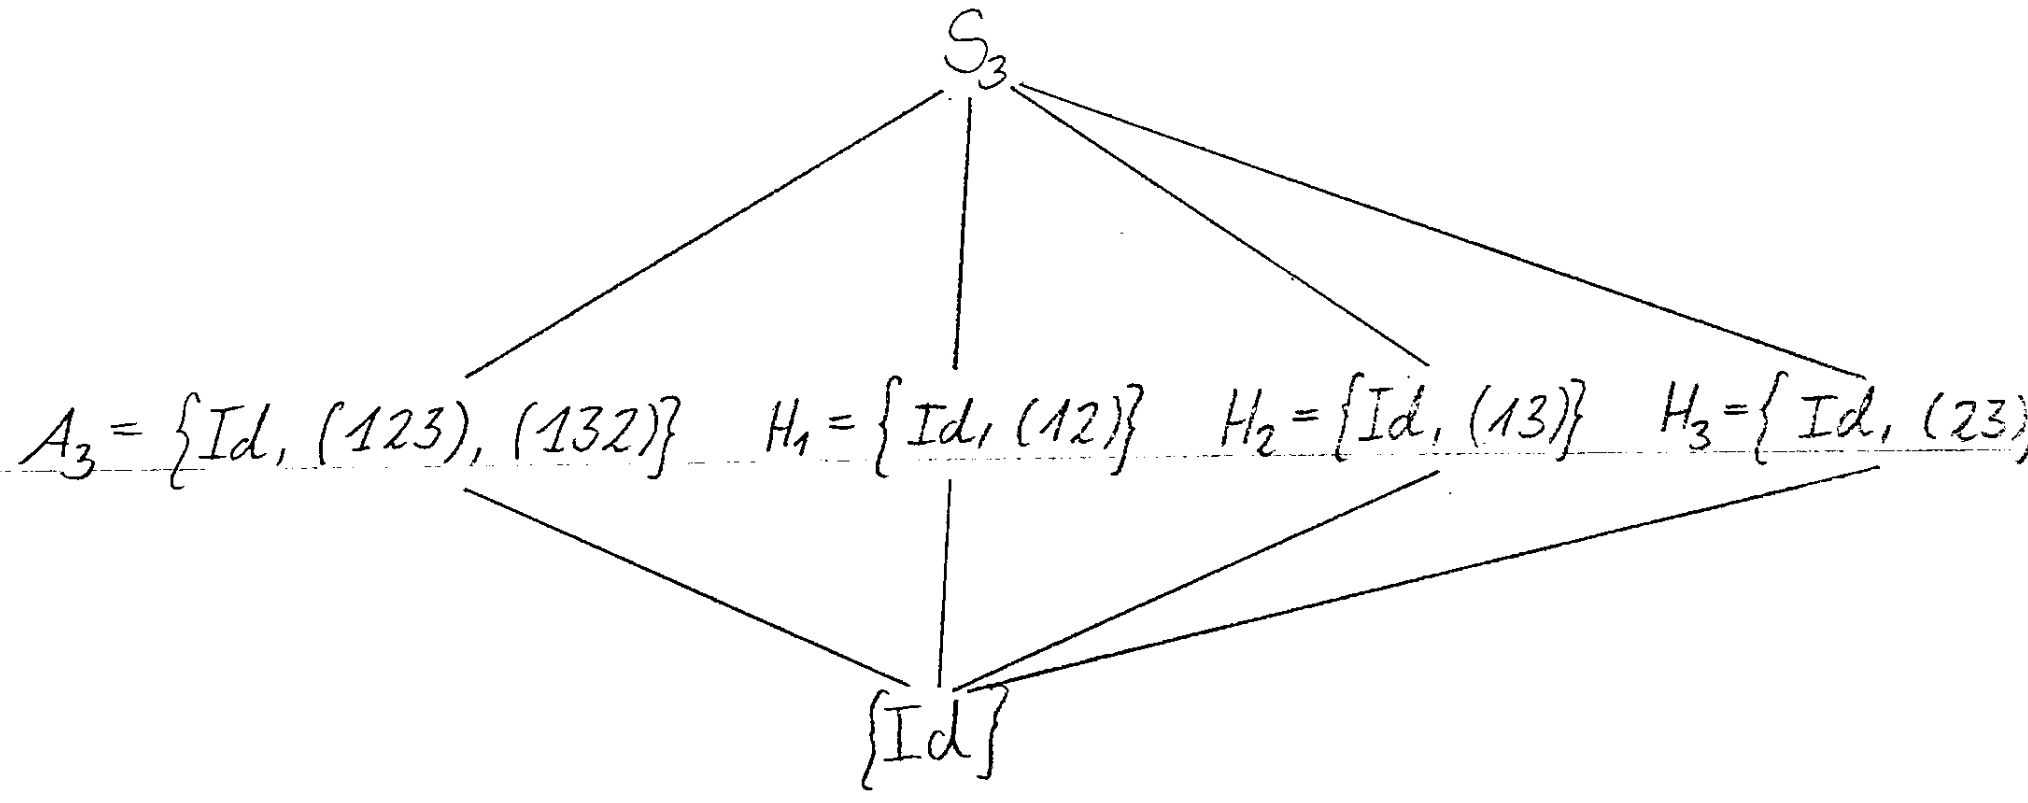
\includegraphics[scale=0.2]{images/beispiel1_15-4}
		\end{center}
		
		Es gilt $A_3 \unlhd S_3$. $H_1, H_2, H_3$ sind jedoch keine Normalteiler, da zum Beispiel $(13)H_1(13) = H_3$.
	\end{enumerate}
\end{beispiel}
\begin{satz}\label{satz1_16}
	Sei $G$ eine Gruppe und $H \unlhd G$.
	\begin{enumerate}[label=(\alph*)]
		\item Die Menge $G/H = \{gH \mid g \in G\}$ mit Multiplikation $(aH) \cdot (bH) = (ab)H$ für alle $a,b \in G$ ist eine Gruppe. Sie heißt \textbf{Faktorgruppe} oder \textbf{Quotientengruppe}.
		\item Die Abbildung $\pi \colon G \to G/H$ mit $g \mapsto gH$ ist ein surjektiver Gruppenhomomorphismus mit $\ker(\pi) = H$. $\pi $ heißt \textbf{kanonische Projektion}.
	\end{enumerate}
\end{satz}
\begin{proof}
	\begin{enumerate}[label=(\alph*)]
		\item Die Multiplikation ist wohldefiniert. Sei $aH = a'H$ und $bH = b'H$ bzw. $a^{-1}a' \in H$ und $b^{-1}b' \in H$. 
		
		\underline{Z.z.: $abH = a'b'H$ bzw. $(ab)^{-1} a'b' \in H$.}
		
		\begin{align*}
			(ab)^{-1} a'b' = b^{-1} a^{-1} a' b' = b^{-1} \underbrace{(a^{-1} a')}_{\in H} b \underbrace{(b^{-1} b')}_{\in H} \in H
		\end{align*}
		
		\paragraph{Gruppenaxiome:} 		
		\begin{enumerate}[label={\bfseries(G\arabic*)}]
			\item Multiplikation in $G$ und in $G/H$ assoziativ.
			\item $H$ ist neutrales Element in $G/H$.
			\item Das Inverse zu $gH$ ist $g^{-1}H$.
		\end{enumerate}
		
		\item Für alle $a,b \in G$ gilt 
		\[\pi(ab) = (ab)H = aH \cdot bH = \pi(a)\cdot\pi(b).\]
		Also ist $\pi$ ein Gruppenhomomorphismus mit
		\[\ker(\pi) = \{g \in G \mid gH = H\} = H\]
	\end{enumerate}
\end{proof}
\begin{beispiel}
	Betrachte $n\Z \unlhd \Z$ für $n \in \N$ mit
	\[\faktor{\Z}{n\Z} = \{n\Z, 1 + n\Z, \dots, (n-1) + n\Z\} =: \Z_n,\]
	wobei $(a + n\Z) + (b + n\Z) = (a + b) + n\Z$. Statt $a + n\Z$ schreiben wir auch $\bar{a}$.
	
	Wir können auch Normalteiler in $\Z/n\Z$ betrachten, zum Beispiel
	\[H = \{\bar{0}, \bar{3}\} \unlhd \Z_6.\]
	$H$ ist offensichtlich Untergruppe und auch noch Normalteiler, da $\Z_6$ abelsch ist. Es gilt
	\[\faktor{\Z_6}{H} = \{H, \bar{1} + H, \bar{2} + H\} \cong \Z_3\]
\end{beispiel}

\begin{prop}\label{prop1_18}
	Sei $H \leq G$ eine Untergruppe. Dann gilt $H \unlhd G$ genau dann, wenn $H$ Kern eines Gruppenhomomorphismus ist, der in $G$ startet.
\end{prop}
\begin{proof}
	\glqq{}$\Rightarrow$\grqq: Folgt aus Satz \ref{satz1_16} (b).
	
	\glqq{}$\Leftarrow$\grqq: Sei $\varphi \colon G \to G'$ Gruppenhomomorphismus und $H = \ker(\varphi)$. Nach Beispiel \ref{beispiel1_6} (6) ist $H \leq G$ Untergruppe. Sei nun $g \in G$ und $h \in H$. Dann gilt
	\[\varphi(ghg^{-1}) = \varphi(g) \varphi(h) \varphi(g)^{-1} = \varphi(g) 1_{G'} \varphi(g)^{-1} = 1_{G'}\]
	Es folgt $gHg^{-1} \subseteq H$ und $H \unlhd G$ ist Normalteiler nach Bemerkung \ref{rem1_14}.
\end{proof}
\begin{beispiel}\label{beispiel1_19}
	\begin{enumerate}[label=(\arabic*)]
		\item Nach Beispiel \ref{beispiel1_8} ist $\sgn \colon S_n \to (\{-1,1\}, \cdot)$ für $n > 1$ ein surjektiver Gruppenhomomorphismus. Nach Beispiel \ref{beispiel1_15} (3) gilt
		\[\faktor{S_n}{\ker(\sgn)} = \faktor{S_n}{A_n} = \{A_n, \pi A_n\},\]
		wobei $\sgn(\pi) = -1$. Insbesondere gilt 
		\[\faktor{S_n}{\ker(\sgn)} \cong \Z_2 \cong (\{-1, 1\}, \cdot) = \im(\sgn).\]
		\item Sei $\varphi \colon \R\setminus\{0\}$ mit $x\mapsto |x|$. Dann ist $\varphi$ ein Gruppenhomomorphismus mit $\ker(\varphi) =\{\pm1\}$ und $\im(\varphi) = \R_{>0}$.
		
		Es gilt
		\[\faktor{\R \setminus \{0\}}{\ker(\varphi)} = \faktor{\R \setminus \{0\}}{(\{-1, 1\}, \cdot)} \cong \R_{>0} = \im{\varphi}\]
		
		\item Nach Beispiel \ref{beispiel1_6} (1) ist $\det \colon \GL_n(K) \to K\setminus\{0\}$ ein surjektiver Gruppenhomomorphismus. Es gilt $\ker(\det) = \SL_n(K)$, sowie
		\[\faktor{\GL_n(K)}{\ker(\det)} = \faktor{\GL_n(K)}{\SL_n(K))} \cong K\setminus\{0\} = \im(\det).\]
		Anstatt diesen Isomorphismus explizit nachzuprüfen, beweisen wir
	\end{enumerate}
\end{beispiel}
\begin{satz}[Homomorphiesatz]\label{satz1_20}
	Sei $\varphi \colon G \to H$ ein Gruppenhomomorphismus. Dann gilt
	\[\faktor{G}{\ker(\varphi)} \cong \im(\varphi).\]
	Insbesondere gilt $|G| = |\ker(\varphi)| \cdot |\im(\varphi)|$ für $G$ endlich.
\end{satz}
\begin{proof}
	Betrachte die Abbildung $\bar{\varphi} \colon G/\ker(\varphi) \to \im(\varphi)$ mit $g\ker(\varphi) \mapsto \varphi(g)$. 
	
	$\bar{\varphi}$ ist wohldefiniert, da für $g\ker(\varpi) = g'\ker(\varphi)$ gilt: Es existiert ein $x \in \ker(\varphi)$ mit $g = g'x$ und somit 
	\[\varphi(g) = \varphi(g'x) = \varphi(g')\varphi(x) = \varphi(g') 1_H = \varphi(g')\]
	
	$\bar{\varphi}$ ist Gruppenhomomorphismus, da für $g, g' \in G$ gilt:
	\[\bar{\varphi}(g\ker(\varphi) g'\ker(\varphi)) = \bar{\varphi}(gg'\ker(\varphi)) = \varphi(gg') = \varphi(g) \varphi(g') = \bar{\varphi}(g\ker(\varphi)) \bar{\varphi}(g'\ker(\varphi))\]
	$\bar{\varphi}$ ist nach Konstruktion surjektiv.
	
	$\bar{\varphi}$ ist injektiv, da aus $\bar{\varphi}(g\ker(\varphi)) = \varphi(g) = 1_H$ folgt, dass $g \in \ker(\varphi)$ und somit $g\ker(\varphi) = \ker(\varphi) = 1_{(G/\ker(\varphi))}$ (siehe Beispiel \ref{beispiel1_6} (6)). $\bar{\varphi}$ ist also ein Gruppenisomorphismus, so dass
	\[\faktor{G}{\ker(\varphi)} \cong \im (\varphi).\]
	Für endliche Gruppen $G$ folgt schließlich mit Satz \ref{satz1_11}
	\[|G| = |\ker(\varphi)| \cdot |\im(\varphi)|.\]
\end{proof}

\begin{satz}[Isomorphiesätze]\label{satz1_21}
	Sei $G$ eine Gruppe und $H_1, H_2 \leq G$ Untergruppen.
	\begin{enumerate}[label=(\alph*)]
		\item Ist $H_1 \unlhd G$ Normalteiler, so gilt $H_1H_2 = H_2H_1 \leq G$ und
		\[\faktor{H_1H_2}{H_1} \cong \faktor{H_2}{(H_1 \cap H_2)}.\]
		\item Sind $H_1, H_2 \unlhd G$ Normalteiler mit $H_1 \leq H_2 \leq G$, so gilt
		\[\faktor{G/H_1}{H_2/H_1} \cong \faktor{G}{H_2}\]
	\end{enumerate}
\end{satz}
\begin{proof}
	\begin{enumerate}[label=(\alph*)]
		\item Da $H_1 \unlhd G$, gilt $h_2 H_1 = H_1 h_2$ für alle $h_2 \in H_2$. Somit $H_1H_2 = H_2H_1$. $H_1H_2$ ist Untergruppe, da $1_G \in H_1H_2$ und daher $1_G = 1_G 1_G \in H_1$. Für $h_1, h'_1 \in H$ und $h_2, h'_2 \in H_2$ gilt 
		\[(h_1h_2)(h'_1h'_2) = h_1(\underbrace{h_2h'_1}_{\in H_1H_2}) h'_2 \in H_1 H_2 \]
		Für $h_1 \in H_1, h_2 \in H_2$ gilt $(h_1h_2)^{-1} = h_2^{-1} h_1^{-1} \in H_2 H_1 = H_1 H_2$. Da $H_1 \unlhd G$, gilt auch $H_1 \unlhd H_1H_2$.
		
		Betrachte nun den Homomorphismus
		\begin{center}
			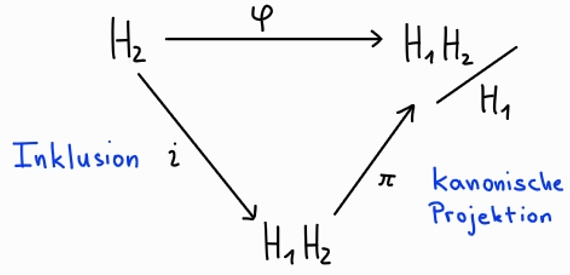
\includegraphics[scale=0.8]{images/2024-10-28_g1}
		\end{center}
		mit $\varphi(h_2) = h_2H_1$. Dann gilt
		\[\ker(\varphi) = \{h_2 \in H_2 \mid h_2 H_1 = H_1\} = H_1 \cap H_2\]
		Da $\varphi$ nach Konstruktion surjektiv, (nutze $H_1 H_2 = H_2 H_1$), folgt mit Satz \ref{satz1_20}
		\[\faktor{H_2}{H_1 \cap H_2} = \faktor{H_2}{\ker(\varphi)} \cong \im(\varphi) = \faktor{H_1H_2}{H_1}.\]
		\item Nach Voraussetzung gilt $H_1 \unlhd H_2$. Die Faktorgruppe $H_2 / H_1$ wird zur Untergruppe von $G/H_1$. Es gilt sogar $H_2/H_1 \unlhd G/H_1$, da für alle $g \in G, h_2 \in H_2$ gilt:
		\[gH_1 h_2H_1 g^{-1} H_1 = \underbrace{gh_2g^{-1}}_{\in H_2, \text{ da } H_2 \unlhd G} H_1.\]
		Betrachte nun den Homomorphismus
		\begin{center}
			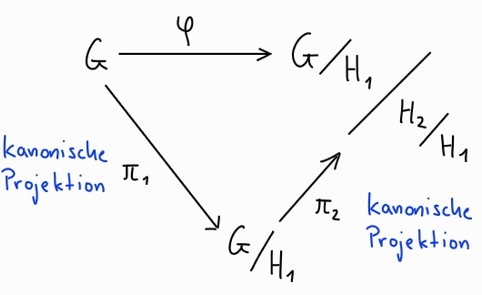
\includegraphics[scale=0.8]{images/2024-10-28_g2}
		\end{center}
		mit $\varphi(g) = gH_1(H_2/H_1)$. Dann gilt
		\[\ker(\varphi) = \{g \in G \mid gH_1 \in \faktor{H_2}{H_1}\} = H_2.\]
		Da $\varphi$ nach Konstruktion surjektiv ist (als Komposition surjektiver Abbildungen), folgt wieder mit Satz \ref{satz1_20}:
		\[\faktor{G}{H_2} = \faktor{G}{\ker(\varphi)} \cong \im(\varphi) = \faktor{G/H_1}{H_2 /H_1}.\]
	\end{enumerate}
\end{proof}
\begin{beispiel}
	\begin{enumerate}[label=(\arabic*)]
		\item Sei $G = \Z$, $H_1 = 3\Z \unlhd G$ und $H_2 = 5\Z \unlhd G$. Dann ist $H_1 \cap H_2 = 15\Z$ und $H_1 + H_2 = \Z$, da $1 = 5(-1) + 3 \cdot 2.$ Satz \ref{satz1_21} (a) liefert
		\[\Z_3 = \faktor{\Z}{3\Z} = \faktor{H_1 + H_2}{H_1} \cong \faktor{H_2}{H_1 \cap H_2} = \faktor{5\Z}{15\Z}.\]
		\item Sei $G = \Z$, $H_1 = mn\Z \unlhd G$ und $H_2 = m\Z \unlhd G$ für $m,n \in \N$. Dann liefert Satz \ref{satz1_21} (b)
		\[\Z_m = \faktor{\Z}{m\Z} = \faktor{G}{H_2} \cong \faktor{G/H_1}{H_2/H_1} = \faktor{\Z/mn\Z}{m\Z/mn\Z}.\]
 	\end{enumerate}
\end{beispiel}

Wie sehen Untergruppen von Faktorgruppen aus? Im Beweis von Satz \ref{satz1_21} (b) haben wir verwendet, dass für eine Gruppe $G$ mit $N \unlhd G$ und $N \leq H \leq G$ gilt:
\[\faktor{H}{N} \leq \faktor{G}{N}.\]
Der Beweis zeigt zudem, dass $H \unlhd G \;\Leftrightarrow\; H/N \unlhd G/N$. 

\begin{center}
	\Large{\textit{Sind alle Untergruppen von $G/N$ von dieser Form?} -- \textbf{Ja!}}
\end{center}

\begin{satz}\label{satz1_23}
	Die Abbildung $\{H \leq G \mid N \leq H\} \to \{\text{Untergruppen von } G/N\}$ mit $H \mapsto H/N$ ist bijektiv.
\end{satz}
\begin{proof}
	Betrachte die kanonische Projektion $\pi \colon G/N$ mit $g \mapsto gN$. Ist $H' \leq G/N$ eine Untergruppe, so gilt 
	\[N \leq \pi^{-1}(H') = \{g \in G \mid \pi(g) \in H'\} \leq G\]
	\begin{itemize}
		\item $g \in N \;\Rightarrow\; \pi(g) = 1_{G/N} \in H'$, also $g \in \pi^{-1}(H')$. Insbesondere $1_G \in \pi^{-1}(H')$.
		\item $g_1, g_2 \in \pi^{-1}(H') \;\Rightarrow\; g_1g_2 \in \pi^{-1}(H')$, da $\pi(g_1g_2) = \underbrace{\pi(g_1)}_{\in H'}\underbrace{\pi(g_2)}_{\in H'} \in H'$.
		\item $g \in \pi^{-1}(H') \;\Rightarrow\; g^{-1} \in \pi^{-1}(H')$, da $\pi(g^{-1}) = \pi(g)^{-1} \in H'$.
	\end{itemize}
	Die Umkehrabbildung zur gegebenen Abbildung in der Aussage liefert die Zuordnung $H' \mapsto \pi^{-1}(H')$, da 
	\[\faktor{\pi^{-1}(H')}{N} = H' \quad\text{sowie}\quad \pi^{-1}(H/N) = H\]
\end{proof}

\begin{rem}\label{rem1_24}
	Die Bijektion in Satz \ref{satz1_23} ist inklusionserhaltend und zeigt, dass die kanonische Projektion $\pi \colon G \to G/N$ einen Isomorphismus von Untergruppenverbänden induziert:
	\begin{center}
		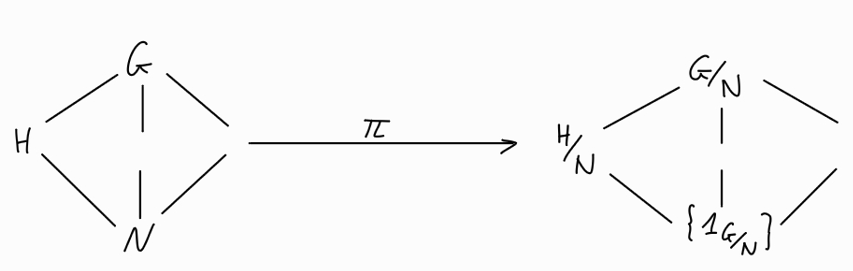
\includegraphics[scale=0.8]{images/2024-10-28_g3}
	\end{center}
\end{rem}